\chapter{Framework Instantiation}
\label{chap:fw-inst}
\index{Framework Instantiation}

%%%%%%%%%%%%%%%%%%%%%%%%%%%%%%%%%%%%%%%%%%%%%%%%%%%%%%%%%%%%%%%%%%%%%%%%%%%%%%%%

In this chapter, we are going to describe in detail how we create an instance
of the framework we proposed in \autoref{chap:fw-design}. We start with the
implementation decisions by explaining why we choose the selected techniques
followed by the project structure used during the implementation time.
Then for each frozen spot introduced in \autoref{sec:fw-design-core} and
\autoref{sec:fw-design-spec}, we describe our instantiation process and the
essential implementation detail.


\section{Implementation Decision}
\label{sec:fw-inst-impl}

In \autoref{sec:fw-design-why}, we stated why choosing the framework
solution. For a programming problem, if we just want to solve it and only it 
specifically, what we need may be just a piece of program. But if we want to
provide a solution in general, it may require extra works and become more
complex. The framework approach aims at providing a general solution, so for
sure its complexity is higher and its development will become more difficult
than the usual approach.
Under such a situation, it is important to make decisions that can enable us to
work efficient and productive. For implementing a framework, what kind of
programming language we are going to use, how to compile the whole framework
with its dependencies and build executable software and how to manage the whole
project efficient and clear are all significant points.

\subsection{Programming Language and Compilation Tool}
\label{sec:fw-inst-lang-ct}

In \autoref{sec:related_work_framework}, a list of currently available software
has been surveyed. From that list we found most of them were written in C++, based
on this fact, to make good used of the existing resources, we
determine to use C++ to develop our framework as well. We can be benefited from
C++ in the following aspects:

\begin{itemize}
    \item Utilizes the existing software maximally.
    \item Obtains faster speed than most of the other programming languages 
    since it is closer to the hardware.
    \item Relatively easier to communicate with other languages since a lot of
    programming language itself were written in C/C++.
\end{itemize}

With these advantages, C++ also has it own limitations. For example, there is
no easy way to manage dependencies when the project becomes complicated.
To address this problem, CMake was selected, which is an open-source cross-platform building tool. By using it, we can build our framework in
Linux, MacOS or any other *nix-based platform with the same command.
Also, with the support of CMake, the end-users can enable the building process
partially which means only compile and build the framework based on their
needs.

\subsection{Framework Layers and Project Structure}
\label{sec:fw-inst-layer-strcut}

In the context of software engineering, a system can be partitioned using the
concept of software layers. Software layers are where each ``layer" of a system
deals with a certain function of a system which, usually, gets more and more
detailed as you burrow down into the layer stack. In our implementation, to separate the responsibility of different modules and specialized
frameworks, we proposed a three-layer software model shown as
\autoref{fig:fw-layers} and assign components into
corresponding layers according to their functionalities, the description of each
layer can be found in \autoref{tab:desc-layer}. With stated logical separation,
in our implemented code base, we also need to structure our code clear and
maintain the modularity of our design. For this purpose, we employ a project
directory structure shown as \autoref{tab:fw-dir}.

\begin{figure}
    \centering
    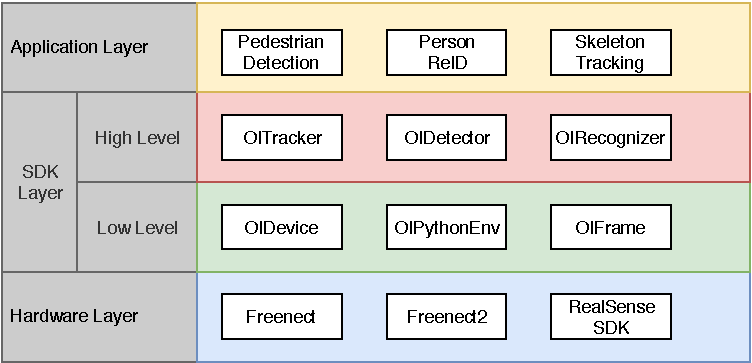
\includegraphics[width=\linewidth]{figures/framework_inst_layers.pdf}
    \caption{Three-layer model for OpenISS framework}
    \label{fig:fw-layers}
\end{figure}

% todo: 需要再重新组织一下 根据上面的图 现在这个不太准确了
\begin{table}
    \resizebox{\textwidth}{!}{%
    \begin{tabular}{ll}
        \hline
        \multicolumn{1}{c}{Layer's Name} & \multicolumn{1}{c}{Description} \\
        \hline
        Application Layer       & \begin{tabular}[c]{@{}l@{}}Provides sample
            usages of the framework for the end-users \\ (application
            developers)\end{tabular} \\ \hline
        SDK Layer (high level)  & \begin{tabular}[c]{@{}l@{}}Provides
            encapsulated functionalities to end-users, hide the \\ complexity
            of
            the implementation
        \end{tabular} \\ \hline
        SDK Layer (low level)   & \begin{tabular}[c]{@{}l@{}}Provides atomic
            APIs to the end-users which enable them to \\
            create custom functionalities based on their own demands
        \end{tabular} \\ \hline
        Hardware Layer          & \begin{tabular}[c]{@{}l@{}}Provides
            encapsulation of the hardware, usually the application \\
            developers
            will not interested in
        \end{tabular}  \\ \hline
    \end{tabular}%
    }
    \caption{Description of the responsibility of different layers}
    \label{tab:desc-layer}
\end{table}

\begin{table}[]
    \begin{tabular}{ll}
        \hline
        Directory Name &
        Description
        \\ \hline
        src       & Contains all the source code of the framework itself
        \\ \hline
        samples   & Contains all the source code of the application level
                    samples
        \\ \hline
        modules   & Contains custom cmake modules for building the framework
        \\ \hline
        python    & Contains all the python modules using by the framework
        \\ \hline
        script    & \begin{tabular}[c]{@{}l@{}}Contains all necessary
                    scripts (e.g. download datasets, \\ configure environment)
                    \end{tabular}
        \\ \hline
    \end{tabular}
    \caption{Directory structure and their functionalities.}
    \label{tab:fw-dir}
\end{table}

\section{Core and Specialized Framework Instantiation}
\label{sec:fw-inst-core-and-spec}

In this section, we describe how we create hot spots for those frozen spots
introduced in \autoref{sec:fw-design-core} and \autoref{sec:fw-design-spec},
the augmented architecture diagram shown as \autoref{fig:fw-inst}.

For the device module in the core framework, we describe how we instantiate it 
to support three different kinds of depth cameras.
For the detector specialized framework, we describe what kind of modification we
made and how we train the YOLO model introduced in
\autoref{sec:related-worked-yolo} and integrate it into our solution as a
detector framework instance.
For the recognizer specialized framework, we describe how we train a person 
ReID network which is a combination of the identification model and triplet 
model explain in \autoref{sec:related-work-re-id-idm} and  
\autoref{sec:related-work-re-id-dism}.
For the tracker specialized framework, we describe how we instantiate it with 
the existing NiTE2 middleware introduced in 
\autoref{sec:related_work_openiss_nite2} implementation.

\begin{figure}
    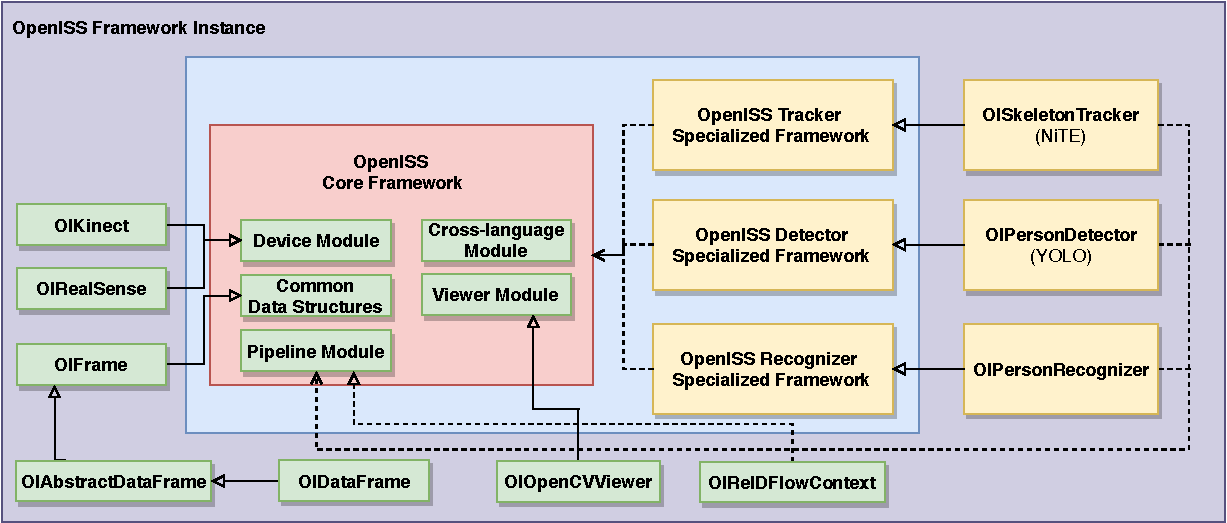
\includegraphics[width=\linewidth]{figures/framework_inst.pdf}
    \caption{Implemented OpenISS framework instance.}
    \label{fig:fw-inst}
\end{figure}

\subsection{Device Module Instantiation}
\label{sec:fw-inst-device}

In \autoref{sec:fw-design-core-device}, we described the design of the device
module within the core framework. To enable our framework to work with
real cameras, we have to instantiate the framework by creating a hot spot for 
the device's frozen spot.
Currently, we plan to support three kinds of devices: Kinect v1, Kinect v2 and
RealSense D435. These devices come from different manufacturers
supported by their own hardware drivers. To combine them within a same set of
APIs, the idea can be illustrated by \autoref{fig:fw-inst-device}. For each
kind of device, we create a concrete class, in our case, will be the class
\texttt{OIKinect} and \texttt{OIRealSense} to wrap the concrete implementation
of the defined functions within the \texttt{OIDevice} abstract class explained
in \autoref{sec:fw-design-core-device}.
Then because of the factory design pattern, what the framework users get from
the factory is a reference with type \texttt{OIDevice}, so they can obtain the
ability accessing the same function definition but with different implementation
from the dynamic dispatch mechanism.

\begin{figure}
    \centering
    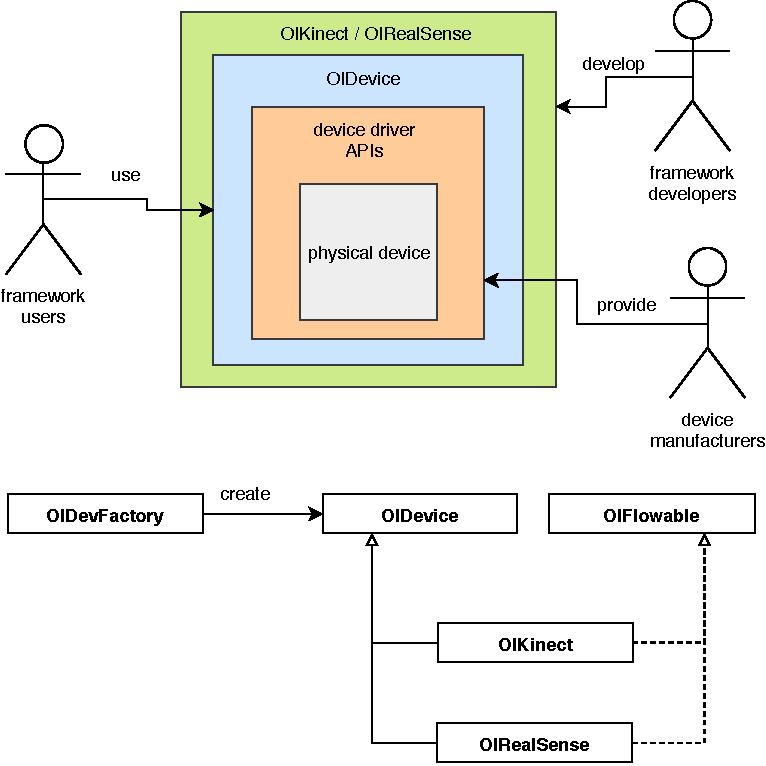
\includegraphics[scale=0.8]{figures/framework_inst_device.pdf}
    \caption{How we instantiate device module of the core framework.}
    \label{fig:fw-inst-device}
\end{figure}

\subsection{Detector Specialized Framework Instantiation}
\label{sec:fw-inst-detector}

\begin{figure}
    \centering
    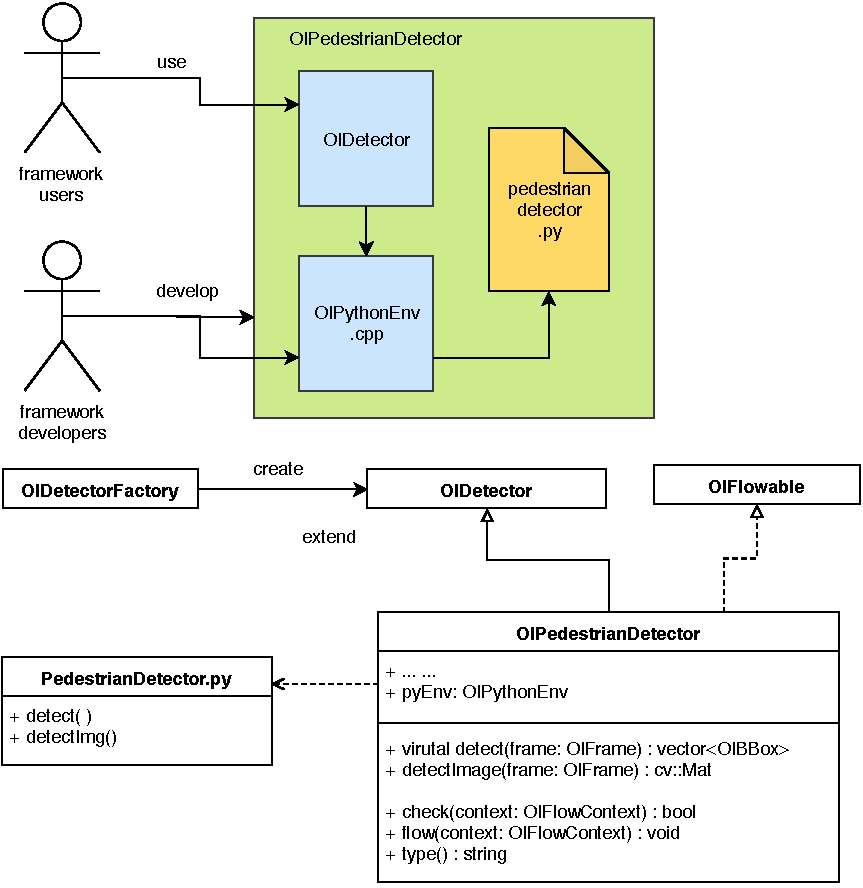
\includegraphics[scale=0.8]{figures/framework_inst_detector.pdf}
    \caption{How we instantiate the detector specialized framework.}
    \label{fig:fw-inst-detector}
\end{figure}

In \autoref{sec:fw-design-spec-detector}, we proposed the design of frozen spot
for a detector specialized framework in general. To achieve person
detection to fulfill our requirement, based on the detector frozen spot, we
create a deep learning-based pedestrian detector hot spot. The overall idea
shown as \autoref{fig:fw-inst-detector}.

We develop a concrete class \texttt{OIPedestrianDetector} which extends the
abstract class \texttt{OIDetector}, serving as a wrapper of the concrete Python
implementation of the YOLO detector. The communication happened here between
C++ and Python is enable by the cross-language module introduced in
\autoref{sec:fw-design-core-cross-lang} from the core framework.
From the users aspect, they don't need to worry about the
how the framework work with various other detectors, but only need to know
the usage of them. For the specialized framework developers, 
with such design, they don't need to know how the cross-language works as well, 
but passing the requested methods or classes name to the \texttt{OIPythonEnv}, 
the cross-language module will handle it for you. It simplifies a lot of works
effectively improving the development process of both the applications and
framework itself.

We previously described the big picture of the detector specialized framework.
In the following paragraph, we will explain in detail how we implement the YOLO
model and reduce its scope from object detection to person detection.
%Recap the background \autoref{sec:intro-background} and requirements
%\autoref{sec:intro-mot-goal} we have, since we are doing performance on the
%stage, real-time data processing is extremely important for our application.
%According to \autoref{sec:related_work_obj_det} we know that
%two stages detector cannot achieve real-time (can only 5 FPS) so our
%selection for object detection model only left with the one-stage detector.
In this thesis, we take \cite{yolov3-keras-github} as a reference and training
facility, re-implement our version of the model since we want to adapt it to
our framework but use the trainer they provided to re-train the model.
The reason why we need to re-train is that the existing YOLO implementation
is used for object detection rather than person detection.
The difference between them is that if you want to make your model be able to
detect more classes of objects the more training time you need to
pay as well as memory space. Since we want to integrate two deep learning-based
approaches (detection and re-identification) in real-time, in such a context,
both time and space complexity are essential to us.

\begin{figure}
    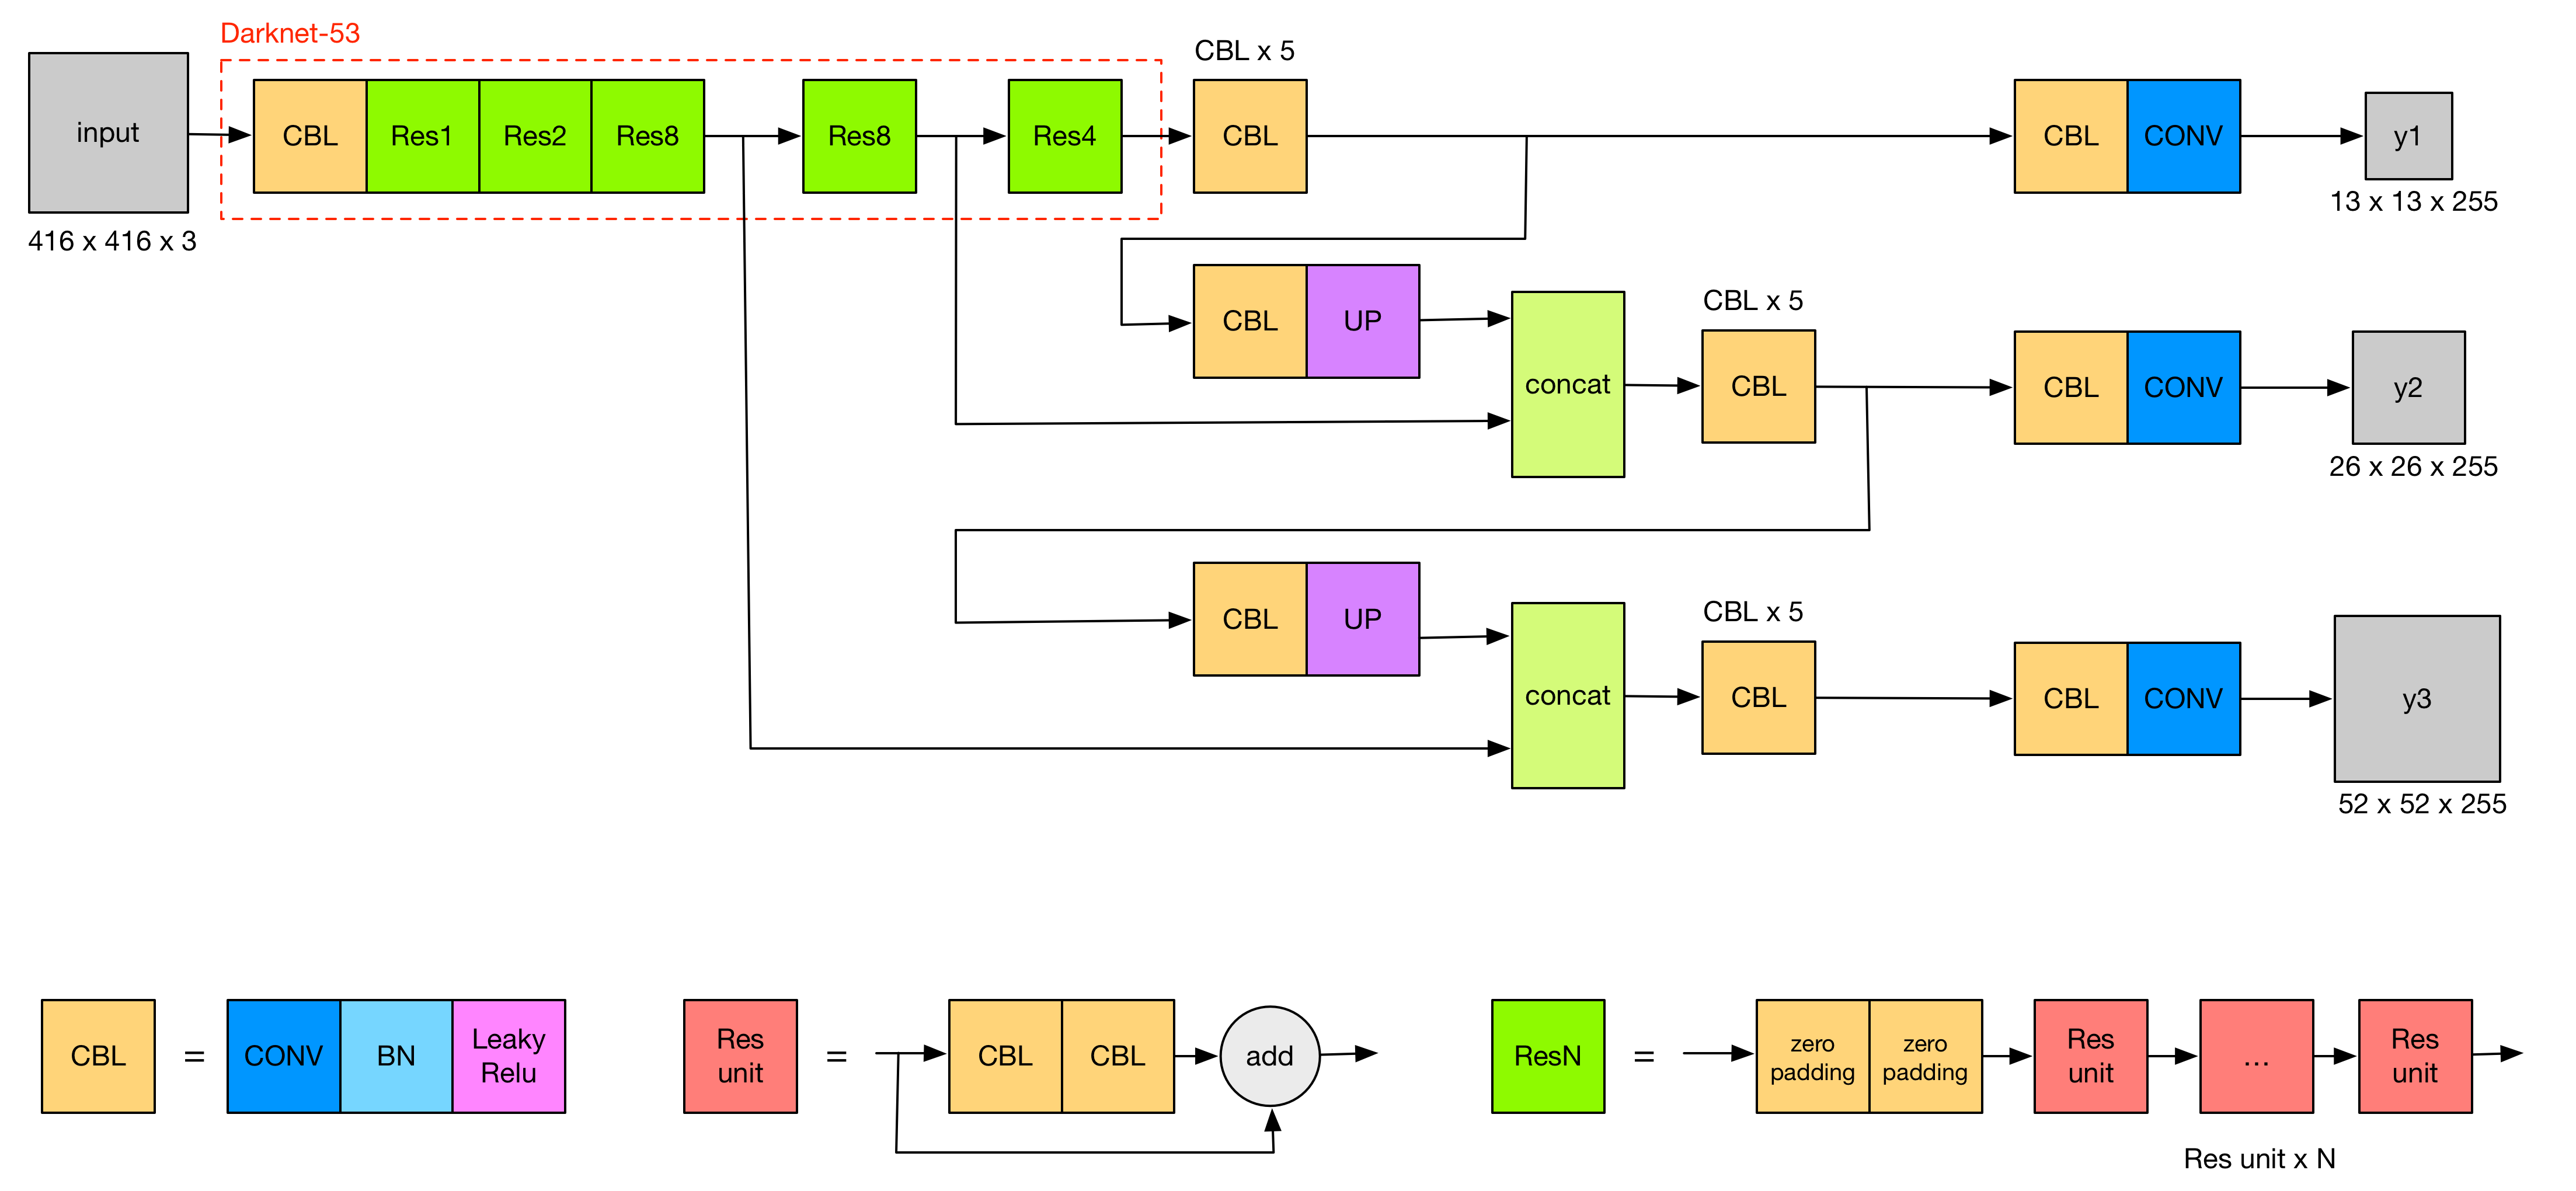
\includegraphics[width=\linewidth]{figures/framework_detector_archit.png}
    \caption{Implemented YOLO v3 architecture}
    \label{fig:fw-detector-archit}
\end{figure}

In our implementation, we follow exactly the same network architecture proposed
in \cite{yolov3-paper-2018} illustrated by \autoref{fig:fw-detector-archit}.
Since there are already tons of pre-trained YOLO model exist, we are not going 
to train it from scratch, but perform some fine-tuning processes 
on a pre-trained model to get the one which can fit to our need.
The full tuning process we employed can be described by the following steps:

\begin{enumerate}
    \item Download the well-trained YOLO model from its official repository.
    \item Convert the model's weight into Keras format from its original
    Darknet format.
    \item Download the VOC2012 dataset and loop over all images in the training
    set annotating the one with person(s) and extracting their corresponding
    bounding boxes information.
    \item Load the converted pre-trained weights then follow the methods
    proposed in the original YOLO v3 paper \cite{yolov3-paper-2018} to 
    fine-tune the model to obtain a person detector rather than an object
    detector.
\end{enumerate}

Since we reduce the complexity of an object detector to a person detector,
we believe that could help to improve the training speed. We are trying to
provide a theoretical analysis to prove it.
According to \cite{yolov3-paper-2018}, there are total 9 anchors which are
obtained by applying K-means cluster algorithm during the training phase. 
These 9 anchors can be divided into 3 groups, each of them is given to final 
feature map with the size $[13, 13, 255]$, $[26, 26, 255]$ and $[52, 52, 255]$ 
respectively. 
So we can calculate that we are going to have:
$13 \times 13 \times 3 + 26 \times 26 \times 3 + 52 \times 52 \times 3=10647$
bounding boxes for each input image. For each bounding box, we need to compute
a probability for each pre-defined classes then multiply the confidence score 
for this box to obtain the final score for one class illustrated by
\autoref{fig:fw-detector-calc}. Take the VOC2012 dataset as
an example, there is a total of 20 classes of object. So for each bounding box,
there will be 20 times multiplication operations. Since we have 105647 boxes,
then it will be $20 \times 10647 = 212940$ operations per input image.
\textbf{
    But if we only care about the person we can reduce the 20 classes to 2
    classes, then the total calculation will be $2 \times 10647 = 21294$ which 
    is one-tenth of the original one. 
}
This can also speed up the non-maximum suppression (NMS) process which could 
help to eliminate overlapped boxes.
In most of the deep learning problem where the training data is normally large,
these modifications will significantly help to reduce the training time.

\begin{figure}
    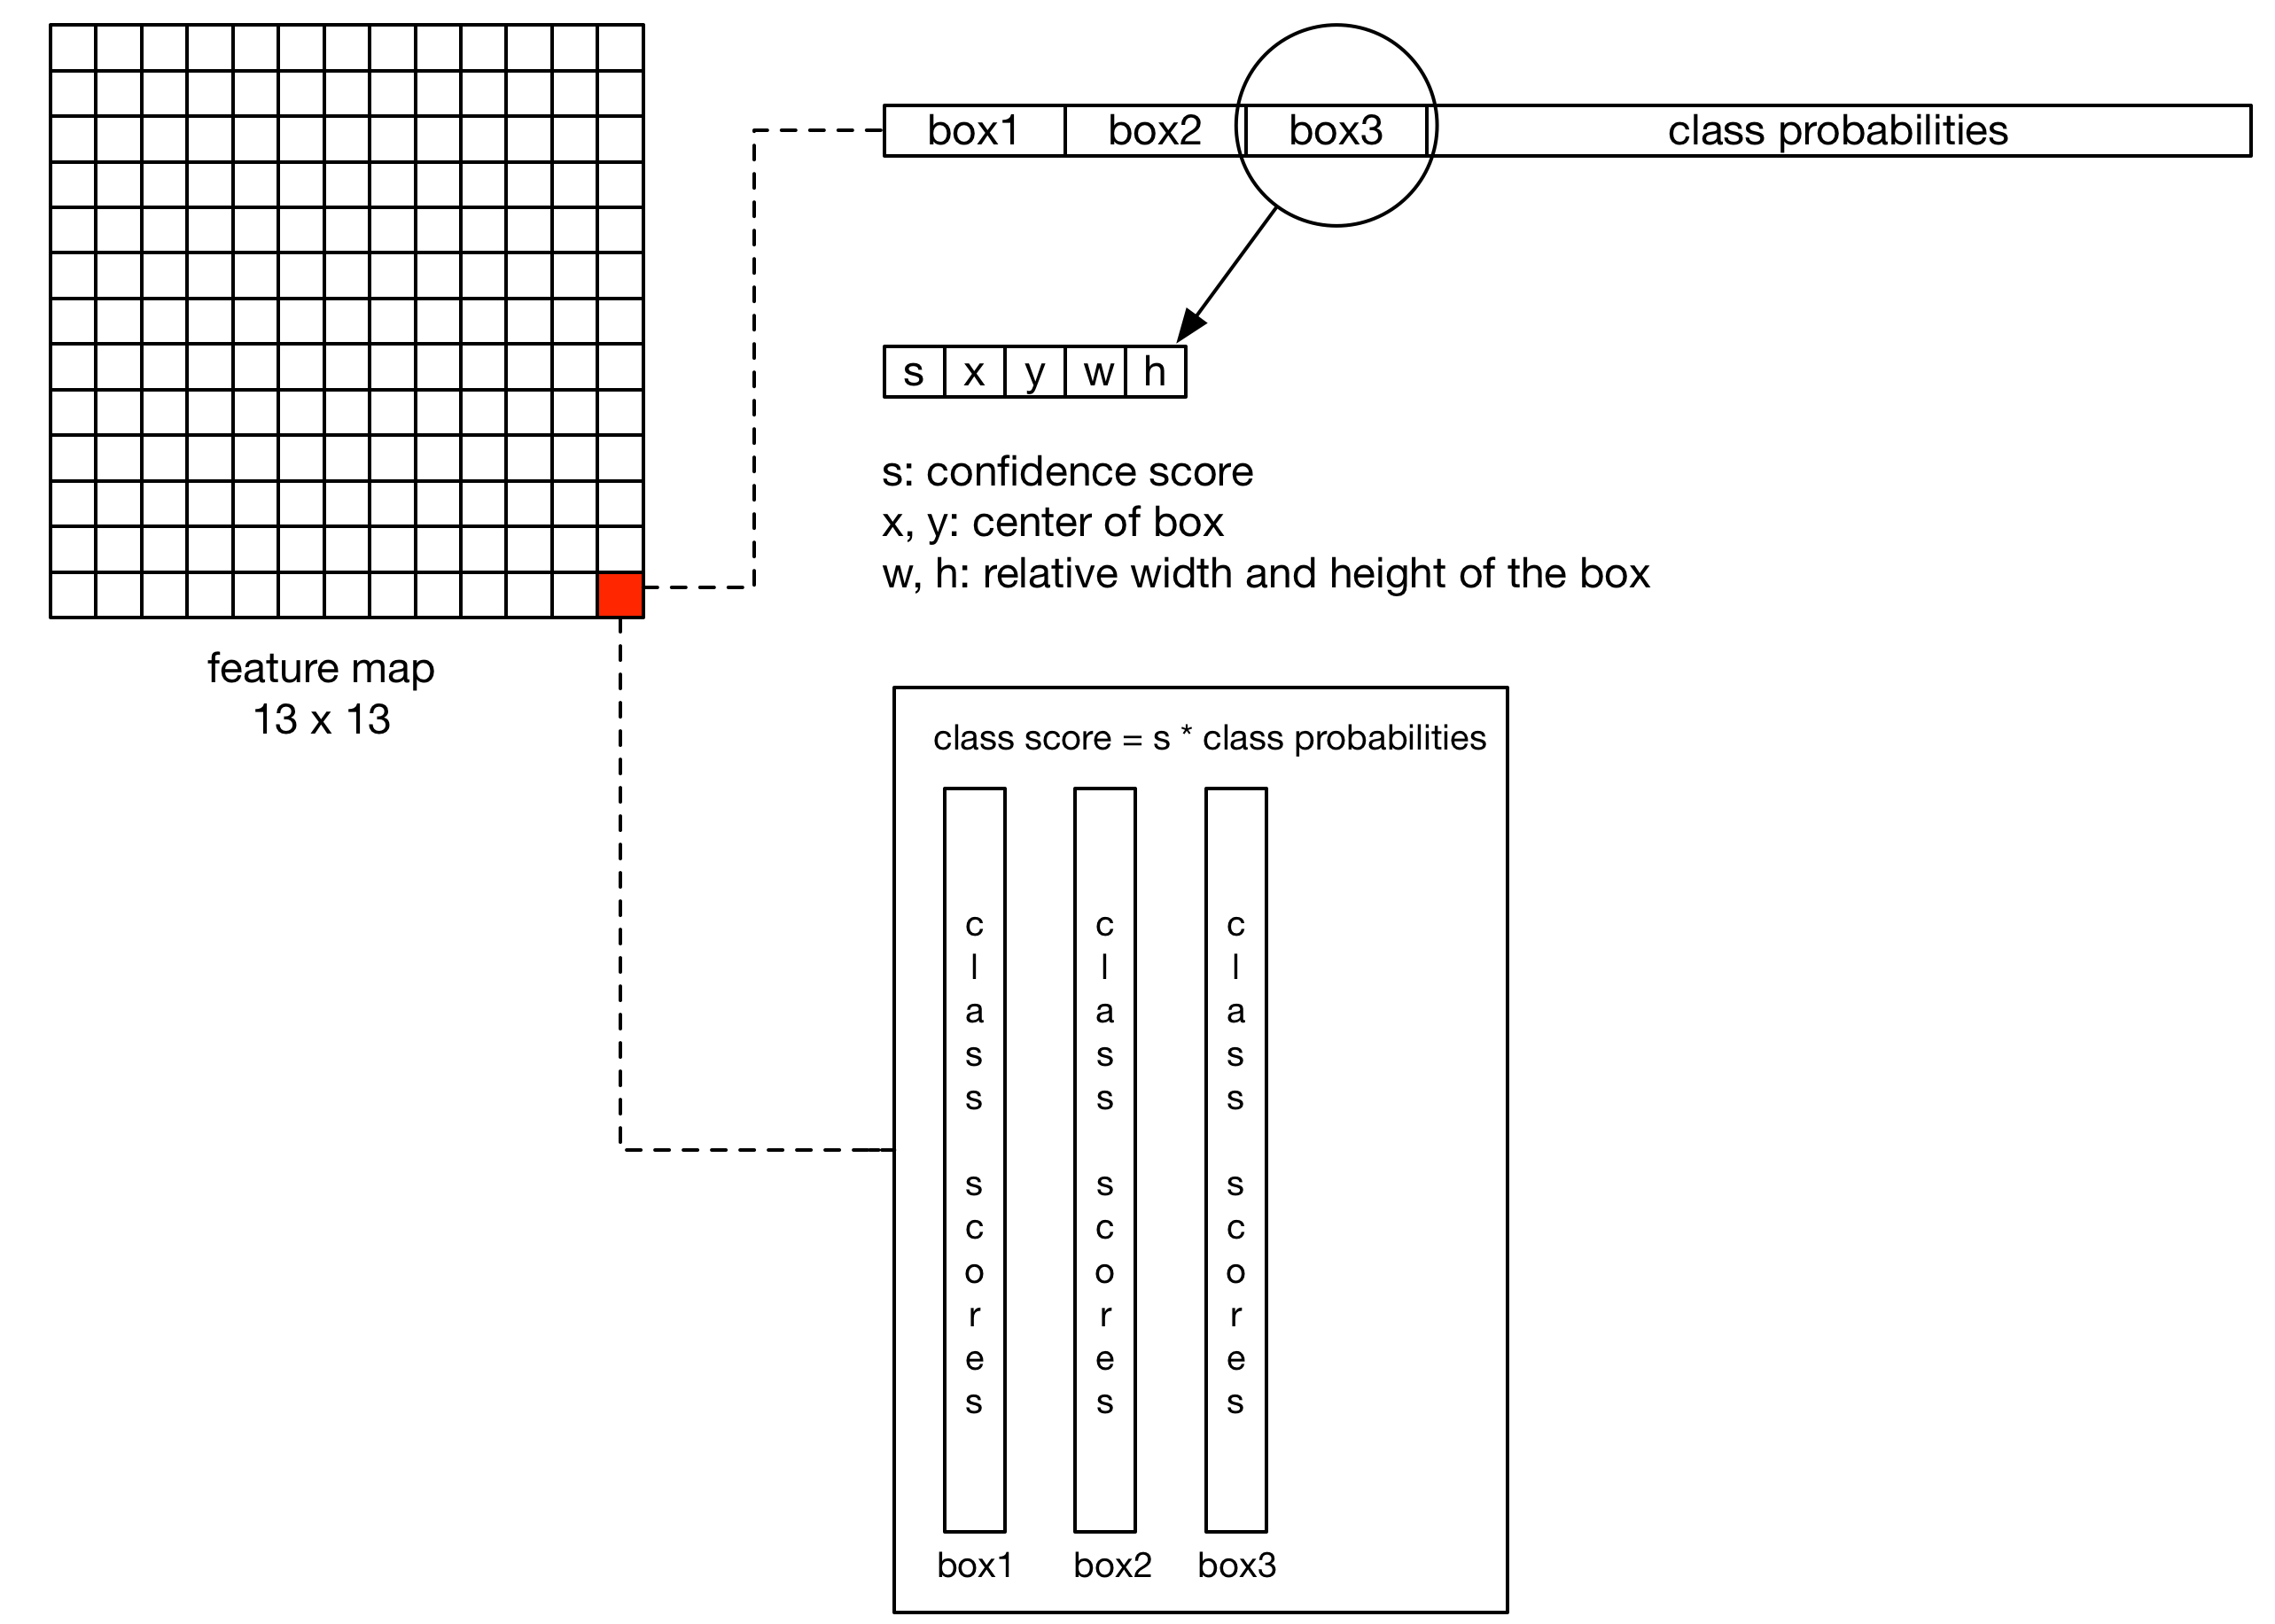
\includegraphics[width=\linewidth]{figures/framework_detector_calc.png}
    \caption{Calculation process of each cell in the feature map.}
    \label{fig:fw-detector-calc}
\end{figure}

Once we have the score for each interested class, we will (1) use a threshold to
filter out the one with a lower score and (2) apply the NMS algorithm to
eliminate the boxes with high ratio overlapping. Assume we still use the
VOC2012 dataset with 20 classes, since we have 10647 boxes, then the class score
can form a $20 \times 10647$ (row $\times$ col) matrix. The procedure can be
described in the following way and visualized by \autoref{fig:fw-detector-nms}.

\begin{enumerate}
    \item Examine all the class scores, select a $threshold$ then set all the
    score lower than $threshold$ to be zero.
    \item Take the class score for the same class from all predictive boxes,
    sort them in a decreasing order.
    \item Mark the box with maximum score as \texttt{bbox\_max}, then use it to
    compare with all the remaining boxes \texttt{bbox\_cur} on the intersection
    over union metric.
    \item if $IoU(\texttt{bbox\_max}, \texttt{bbox\_cur}) > 0.5$ then set the
    score to be zero. Otherwise, keep it unchanged.
\end{enumerate}

\begin{figure}
    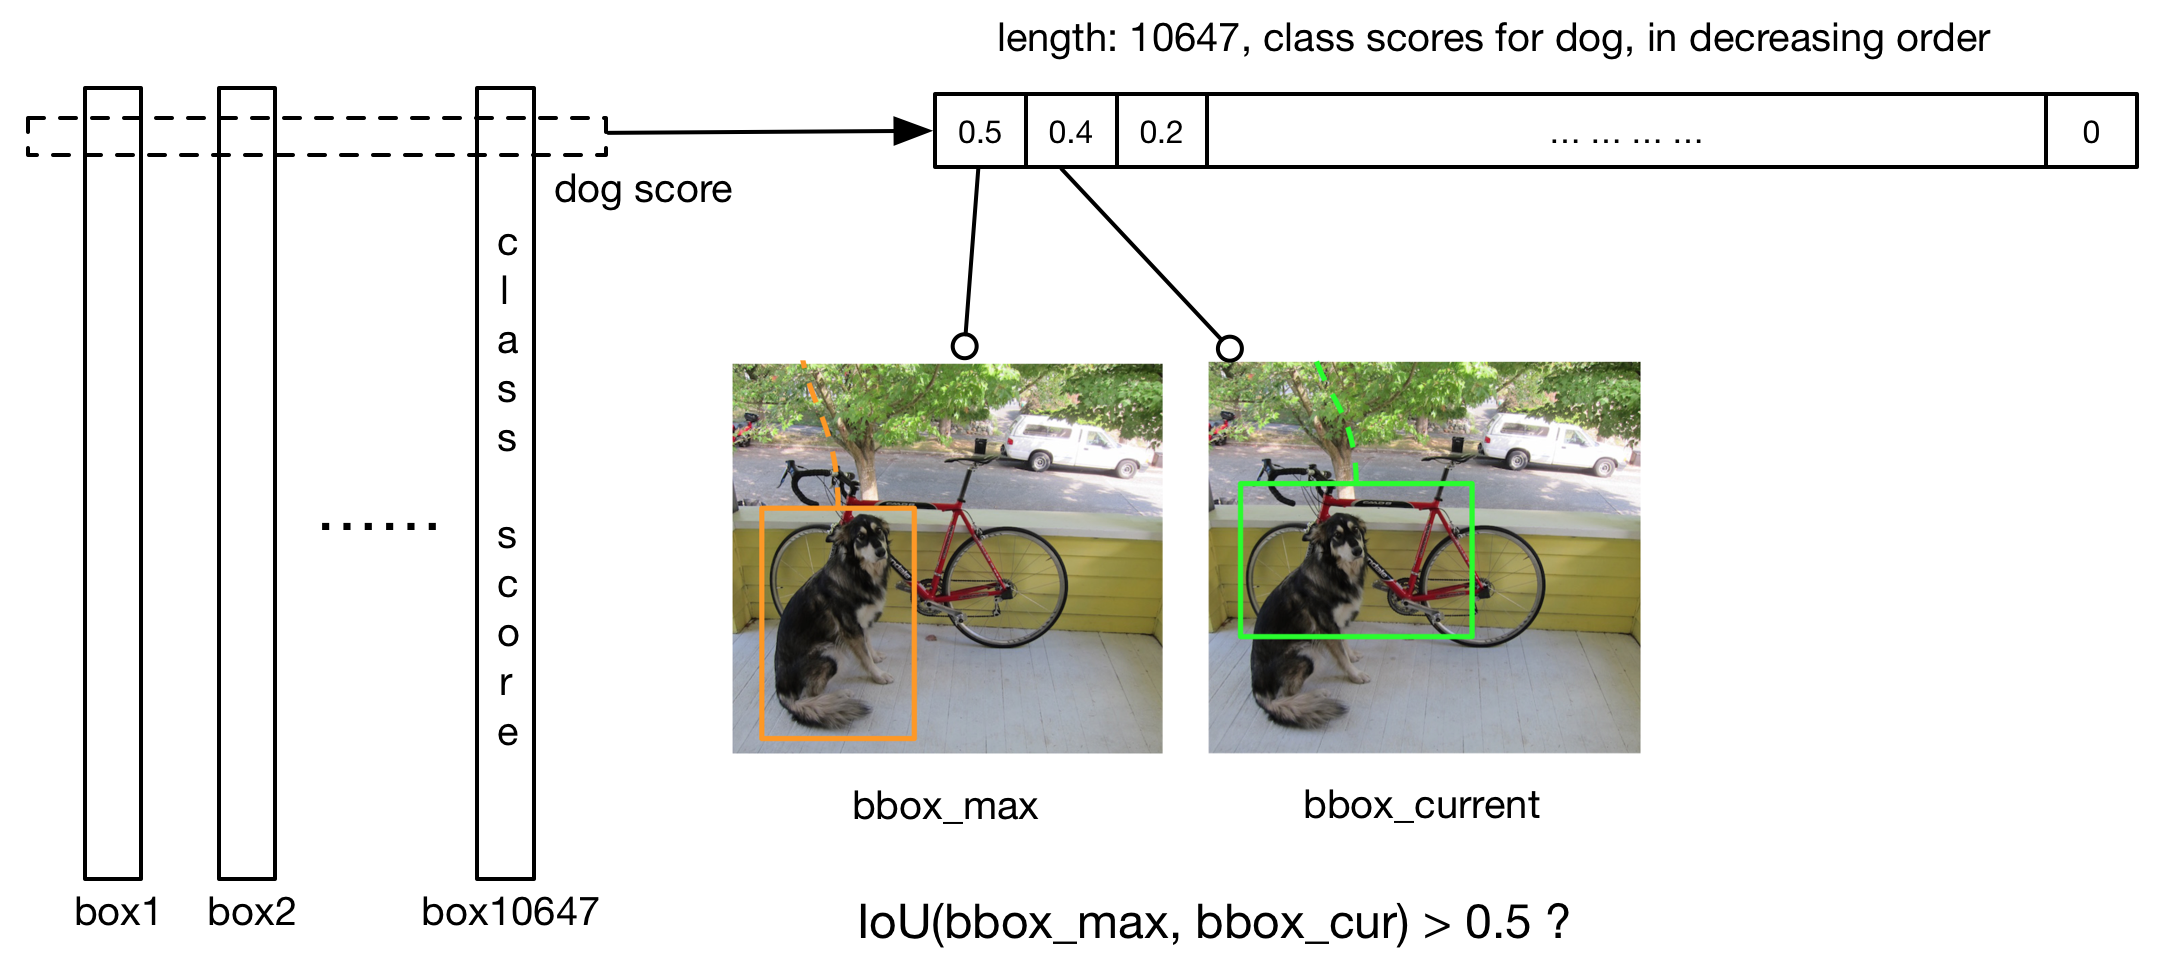
\includegraphics[width=\linewidth]{figures/framework_detector_nms.png}
    \caption{The process of non-maximum suppression.}
    \label{fig:fw-detector-nms}
\end{figure}

\subsection{Recognizer Specialized Framework Instantiation}
\label{sec:fw-inst-recoginzer}

Person recognizer is the most significant component in our specialized
framework, without it we cannot reach our final goal covering the stage with
more than one camera. In \autoref{sec:fw-design-spec-recognizer}, we proposed the
basic architecture of the frozen spot for a common recognizer. For our specific
purpose, we need the capacity to re-identify the same person across multiple
cameras, so what we need is actually a person recognizer instance (hot spot).
Just like the way we did for the detector, we follow the same idea and come up with
the instantiation plan shown as \autoref{fig:fw-inst-recognizer}. The only
difference here is that the database invoked in this case, we have to create
the database first before we use the recognizer, otherwise, there is nothing to
be recognized. There is a variety of ways to create the database, the corresponding
logic should be added into the \texttt{attachDatabase} method. And the way how
to compare the input and the record within the database should be written in
the method \texttt{lookupDatabase}. In this case, we are using a deep
learning-based model, so what we need to is using the model to compute the
descriptor for each given record and store them in the database then compare the
distance between query and gallery descriptors, more detail can be found in
\autoref{fw-recognizer-spec-inference}.

\begin{figure}
    \centering
    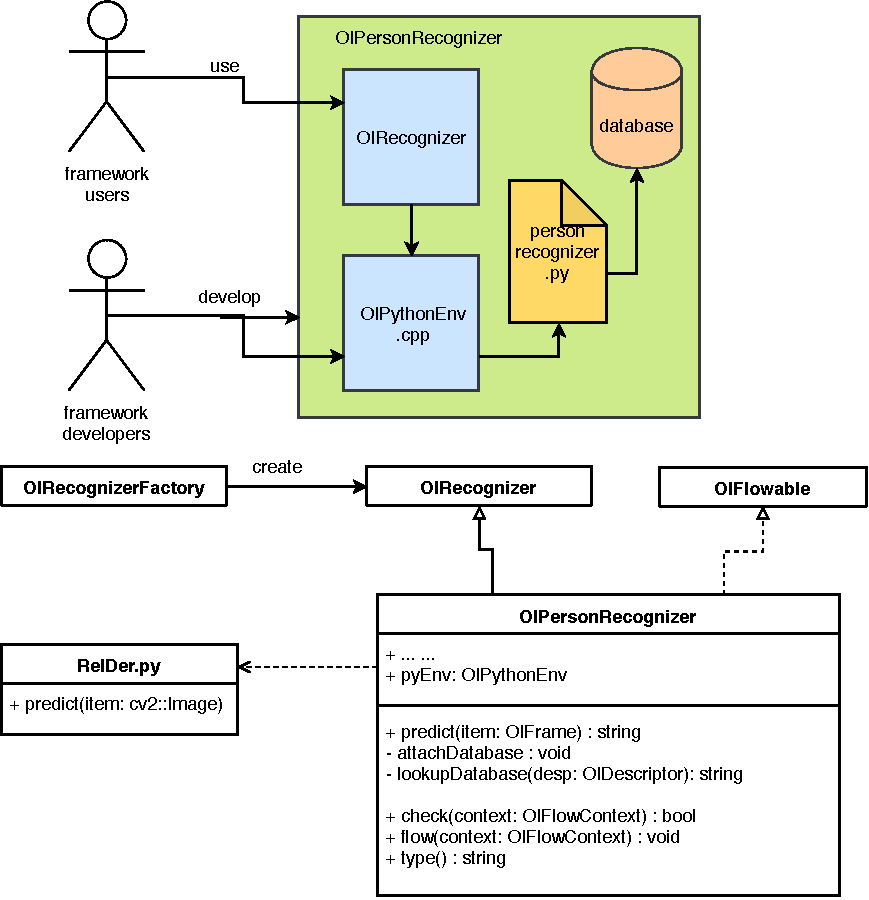
\includegraphics[scale=0.8]{figures/framework_inst_recognizer.pdf}
    \caption{How we instantiate the recognizer specialized framework.}
    \label{fig:fw-inst-recognizer}
\end{figure}

In order to keep the consistency with the person detector and fill the
research gap described in \autoref{sec:related_work_openiss_tf}, our 
implementation of the recognizer is written in Python and built on top of 
TensorFlow and Keras.
In the following paragraph, we will first introduce our network structure, then
explain our training process which includes data pre-processing, loss 
function,  optimizer and some important hyper-parameters.
In the end, we will discuss the methodology which we used to perform inference
by using the trained model.

\subsubsection{Network Architecture}
\label{fw-recognizer-spec-network-arch}

\begin{figure}
    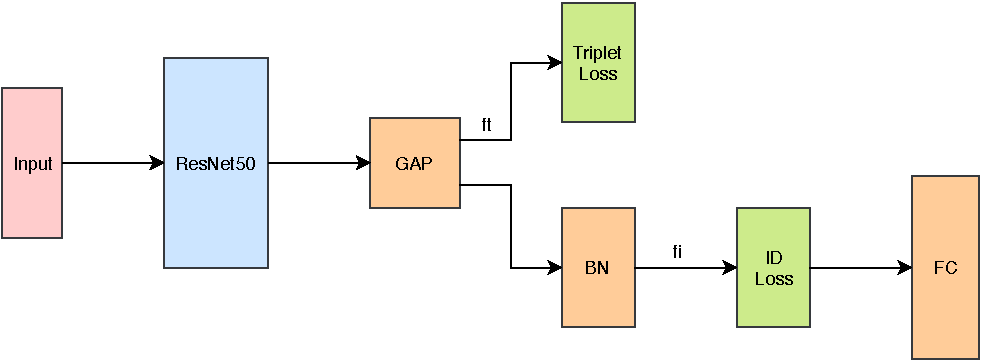
\includegraphics[width=\linewidth]{figures/framework_reid_archit.pdf}
    \caption[Implemented recognizer network architecture]
    {
        Implemented recognizer network architecture.
%        GAP: global average pooling layer, BN: batch normalization
%        layer, FC: fully connected layer.
%        $f_t$: features used to calculate triplet loss,
%        $f_i$: features used for inference.
        The pink color represents input, blue means backbone network, orange
        represents a special layer and green means loss function layer.
    }
    \label{fig:fw-reid-archit}
\end{figure}

We implemented a network architecture shown as \autoref{fig:fw-reid-archit},
which is a combination of the identification model and distance metric-based
model mentioned in \autoref{sec:related_work_re_id}. It employed a Residual-50
network as the feature extractor followed by a global average pooling layer
(GAP) to flatten out the feature vector. Then in one branch, the extracted
feature $f_t$ was sent to calculate the triplet loss while in
the other branch was used to obtain $f_i$ after passing through a batch 
normalization layer (BN) to compute the identification loss. 
In the end, the fully connected
layer (FC) is responsible for classification during the training time.
According to \cite{pcb-and-rpp-for-reid},
if we can get a higher spatial resolution before global pooling by changing the
stride in the last convolutional layer from 2 to 1, which would not affect the
number of parameters, obvious improvement can be obtained. Because of that, we
modified our ResNet50 accordingly. Like most of the deep learning tasks, our
model was also initialized with the weights pre-trained on ImageNet.
From the implementation point of view, it is important
to point out that when we are using any pre-trained weights, we need to make
sure the input image respect to the format of the pre-trained model. In Keras,
this can be done by invoking the \texttt{preprocess\_input} method within the
pre-defined model package.

\subsubsection{Training}
\label{fw-recognizer-spec-train}

As we can see from \autoref{fig:fw-reid-archit}, during the training, our model
will be guided by two loss functions: triplet loss and ID loss.

%\begin{equation}
%    L = L_{triplet} + \beta L_{center} + L_{ID}
%\end{equation}

\begin{equation}
L = L_{triplet} + L_{ID}
\end{equation}

\noindent where $L_{triplet}$ is defined as \autoref{eq:common-triplet-loss},
$L_{ID} = - \mathbf{y} \cdot \log(\mathbf{\hat{y}})$
is the cross-entropy loss.
% and $L_{center} = \frac{1}{2} \sum_{j=1}^{B}
%\norm{f_{t_j} - c_{y_i}}^2_2 $ represents the center loss
%\cite{center-loss-2016}. In our implementation, $\beta$ is set to 0.0005.

Since the training set is too large to fit into memory in one shot,
the mini-batch training strategy was adopted as well as
the sampling method proposed in \cite{in-defense-of-triplet-loss-for-reid-2017}.
For each mini-batch, we randomly select $P$ identities and for each identity 
random $K$ images will be chosen. In our implementation,
$P$ is set to 16 and $K$ is set to 4, which makes the batch size to become 64.
This work is done by the class \texttt{RandomSampler} whose UML diagram shown as
\autoref{fig:fw-sampler-uml}.

In order to prevent overfitting and enhance the generalization ability of the
model, a data augmentation technique named random erasing
\cite{random-erasing-data-augmentation-2017} was applied to each image
individually on-the-fly when constructing each mini-batch of data. Just like its
name suggests, it will randomly replace a portion of the pixel's intensity 
within the image with some random values. 
Besides that three more steps pre-processing
were applied to enlarge the dataset. These pre-processing methods are commonly
used in the image-based deep learning problem, they are implemented in the file
named \texttt{preprocess.py}.

\begin{itemize}
    \item Pad 10 pixels around the image
    \item Randomly crop the image back to the size before padding
    \item Flip the image horizontally with 0.5 probability
\end{itemize}

For the optimizer, we used the build-in Adam algorithm provided by Keras
but with warm-up learning rate setting \cite{learning-rate-warmup-2018}.
Precisely, the learning rate has been scheduled as \autoref{eq:reid-lr}, where 
$t$ is the current epoch. Last but not least, according to
\cite{tricks-and-baseline-for-reid-2019}, they trained their model for 120
epochs and it is sufficient to obtain a good result. Also, from our training
result shown by \autoref{fig:fw-training}, this number is enough for the
model's convergence, so we set our total training epochs to 120 as well.

\begin{equation}
\label{eq:reid-lr}
\operatorname{lr}(t)=\left\{
\begin{array}{ll}
{3.5 \times 10^{-5} \times \frac{t}{10}} & {\text { if } t \leq 10} \\
{3.5 \times 10^{-4}} & {\text { if } 10<t \leq 40} \\
{3.5 \times 10^{-5}} & {\text { if } 40<t \leq 70} \\
{3.5 \times 10^{-6}} & {\text { if } 70<t \leq 120}
\end{array}\right.
\end{equation}

\begin{figure}
    \begin{center}
        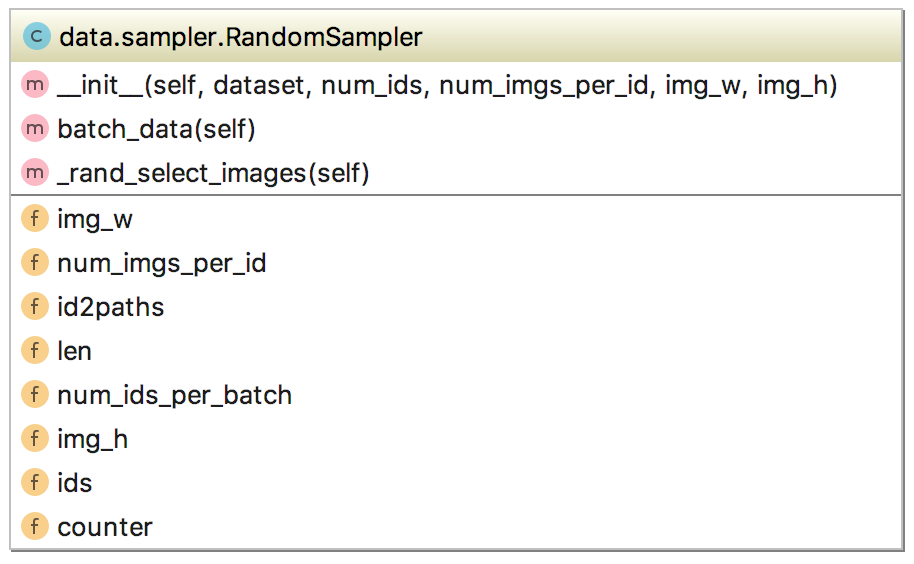
\includegraphics[scale=0.6]{figures/framework_reid_sampler_uml.png}
    \end{center}
    \caption{UML diagram of \texttt{RandomSampler} class}
    \label{fig:fw-sampler-uml}
\end{figure}

From the implementation point of view, the training program can be illustrated by
\autoref{fig:fw-reid-code-overview}. Firstly, we defined a set of configuration
variables and the structure of the model. Then we pass the configuration to the
model, attach it with defined loss functions, optimizer and necessary
callback functions then run the model in training mode. During the training
time, the data will be retrieved from the dataset, sampled by the
\texttt{Sampler}, applied data argumentation by \texttt{DataGen} and wrapped
up to be a Python generator object by \texttt{DataGenWrapper}.

With these setting and after training, the result can be visualized by
\autoref{fig:fw-training}, we can see clearly that the model starts to converge
at around $50^{th}$ epochs. And from the training accuracy figure, we can find
that there is a steep increase between $10^{th}$ and $20^{th}$ epochs.

\begin{figure}
    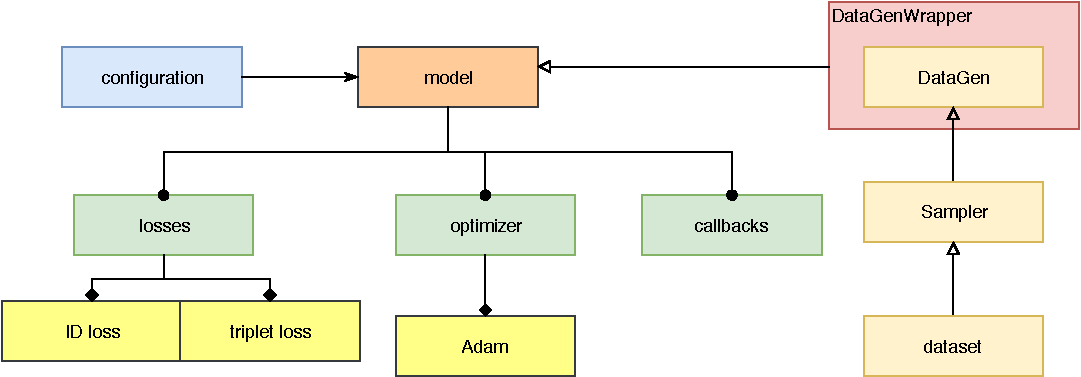
\includegraphics[width=\linewidth]{figures/framework_reid_code_overview.pdf}
    \caption{Code structure of the ReID training program}
    \label{fig:fw-reid-code-overview}
\end{figure}

\begin{figure}
    \begin{subfigure}
        \centering
        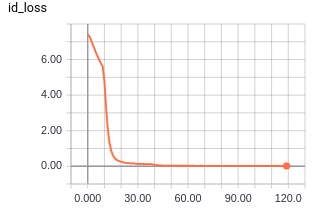
\includegraphics[width=.5\linewidth]{figures/train_id_loss.png}
    \end{subfigure}
    \begin{subfigure}
        \centering
        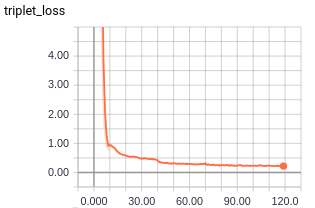
\includegraphics[width=.5\linewidth]{figures/train_triplet_loss.png}
    \end{subfigure}
    \begin{subfigure}
        \centering
        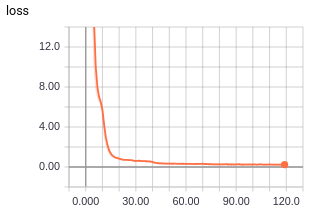
\includegraphics[width=.5\linewidth]{figures/train_loss.png}
    \end{subfigure}
    \begin{subfigure}
        \centering
        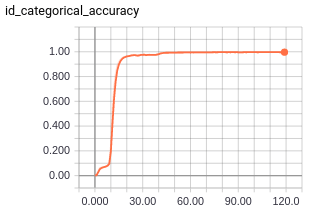
\includegraphics[width=.5\linewidth]{figures/train_acc.png}
    \end{subfigure}
    \caption[Training visualization diagram]
    {Training visualization diagram. upper left: training identification loss
        curve, upper right: training triplet hard loss curve, lower left: total
        training loss curve, lower right: training classification accuracy.}
    \label{fig:fw-training}
\end{figure}

\subsubsection{Inference}
\label{fw-recognizer-spec-inference}

We explained the training process above, let's take a look at the inference
procedure. Assume we have a query image $q$ and a set of gallery images $G$.
The model is denoted by $M$ and the output of model will be $f_i$ then we have:

$$
f_i^{query} = M(q) \:\:\: \text{and} \:\:\: f_i^{G} = M(G)
$$

Once we have the feature descriptor, then for each $f \in f_i^G$  we calculate
the distance $D_i$ between $f$ and $f_i^{query}$:

\begin{equation}
\label{eq:dis-comp}
D_i =  distance(f, f_i^{query}) \:\: f \in f_i^G
\end{equation}

Finally, the gallery image which gives the minima distance will be the one
whose identity needs to be returned:

$$
id = \arg \min(D_i)
$$

If the reader wants to reproduce the result, attention need to be paid on one issue
that the dimension of $f_i^{query}$ and $f_i^G$ are different so when we try
to feed the single query image into the model, we have to explicitly add one
more axis to it.
What's more is that, according to \autoref{eq:dis-comp},  $distance$ function is
used to perform comparison between $f$ and $f_i^{query}$. The most popular
distance function for two vectors comparison are: (1) euclidean distance and (2)
cosine distance. According to \cite{tricks-and-baseline-for-reid-2019}, using
(2) can obtain a better result. Our implementation offers both two
methods, but for simplicity we don't follow exactly the cosine distance
calculation. We have the function \texttt{euclidean(f1, f2)} for the standard
Euclidean distance but \texttt{L2(euclidean(f1, f2))} which is
mathematics equivalent for Cosine distance.

\subsection{Tracker Specialized Framework Instantiation}
\label{sec:fw-inst-tracker}

In the plan of OpenISS framework, there are three kinds of tracker are needed:
skeleton tracker, facial landmark tracker and gesture tracker. In this thesis,
we focus on the skeleton tracker.
Skeleton tracking is the processing of depth image data to establish the
positions of various skeleton joints on a human form. This information can be
useful in many cases, as mentioned in \autoref{sec:related_work_other},
the approach proposed by \cite{rgbd-for-reid} takes skeleton as the starting
point. A lot of research has been conducted in this area and a lot of
methods both conventional and deep learning-based have been developed. We will
not focus on developing our approach but implement one and design it as an
instance of the specialized framework to allow users to integrate others or
develop their own approach easily. \autoref{fig:fw-skeleton} is an example
result from our solution.

\begin{figure}
    \begin{center}
        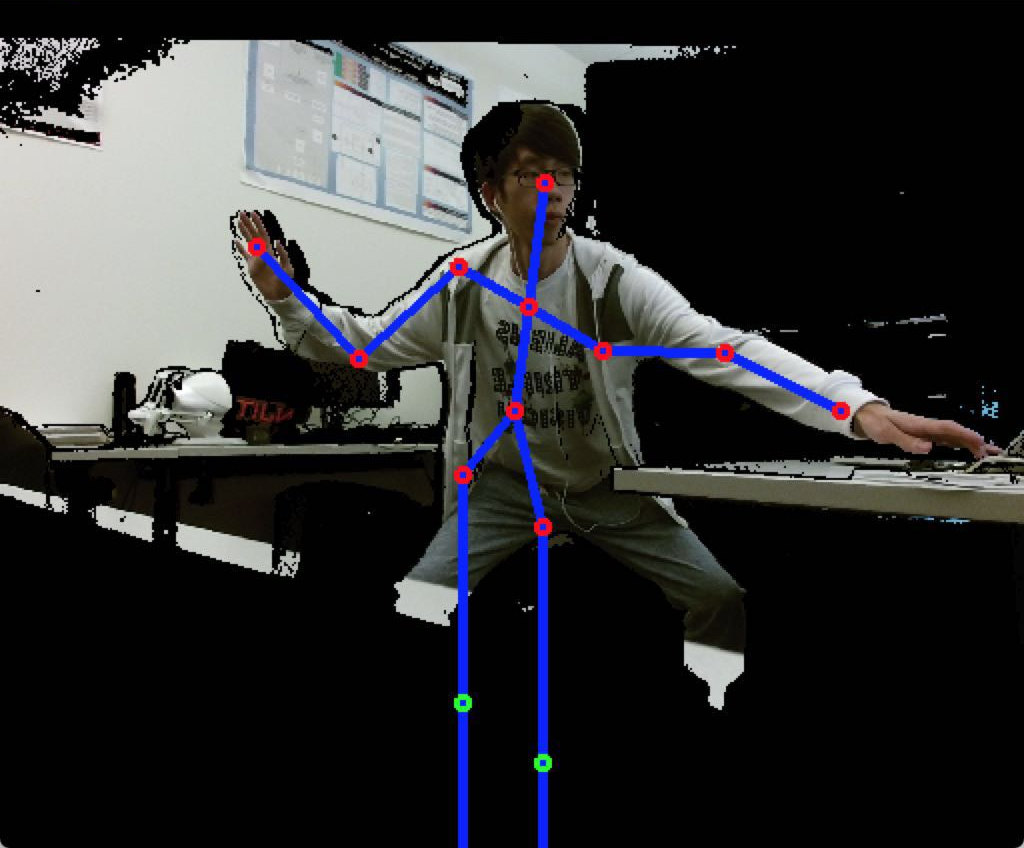
\includegraphics[scale=0.3]{figures/framework_skeleton.png}
    \end{center}
    \caption[An example of skeleton tracking]
    {An example of skeleton tracking, red points represent high
        confidence and green point mean less confidence.}
    \label{fig:fw-skeleton}
\end{figure}

Like what we did for the device abstraction, here we design a similar mechanism
which is a hierarchical architecture shown as \autoref{fig:fw-skeleton-tracker}
that can support real-time skeleton tracking with good extensibility without
any GPU device needed.
From the implementation point of view, firstly, we abstract the common
functionalities of the skeleton tracker to create an abstract superclass
\texttt{OITracker}, which serves as a contract exposed to the users hiding the
complexity.
Since our implementation is based on a middle-ware of OpenNI2 named NiTE2
mentioned in \autoref{sec:related_work_openiss_nite2}. So we create a concrete
subclass which inherited from \texttt{OITracker} named \texttt{OINiTETracker}.
It can be seen as an adapter that adapts the NiTE tracking algorithm to our
framework's data structure.
Let's go deeper, starting from the method \texttt{readFrame(OITrackerFrame)}.
Every time a new frame (image) is read from the device, this method will be
invoked. Its job is to perform skeleton detection to take the data from the
NiTE2's data structure and move them to several OpenISS framework's data
structures which will be eventually packed into \texttt{OITrackerFrame}.
There are three specialized framework specific data holder classes and their
responsibilities listed below:

\begin{itemize}
    \item \texttt{OIUserData}, it contains all the data for each single
    detected skeleton.
    \item \texttt{OIUserMap}, it contains a 2d array with the same resolution
    as the depth image, where the background indicated by 0 and the detected
    skeleton for each person indicated by their user id.
    \item \texttt{OISkeleton}, it contains a hashmap which the key is the joint
    type and the value is the position of that joint.
\end{itemize}

\begin{figure}
    \centering
    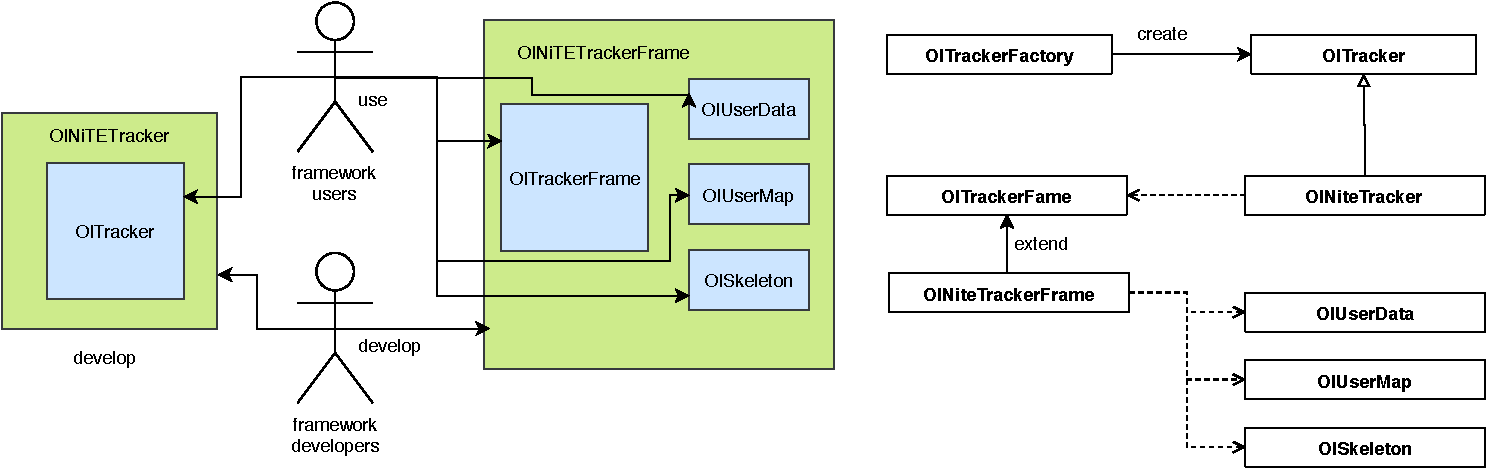
\includegraphics[scale=0.6]{figures/framework_inst_tracker.pdf}
    \caption{How we instantiation tracker specialized framework.}
    \label{fig:fw-skeleton-tracker}
\end{figure}

\subsection{ReID Context Instantiation}
\label{sec:fw-inst-context}

As mentioned in \autoref{sec:fw-design-core-pipeline}, we have the pipeline
module designed in the core framework. In this chapter, we have
\texttt{OISkeletonTracker}, \texttt{OIPedestrianDetector} and
\texttt{OIPersonRecognizer} both implement the \texttt{OIFlowable} interface to
serve as filters within the pipeline. In order to build up a ReID pipeline for
our final goal, what we are still missing is a concrete class for the
\texttt{OIFlowContext} which will be used as the data holder for intermediate
result generated during the execution of the pipeline.
For this purpose, we define a class \texttt{OIReIDFlowContext} which extends
the abstract class \texttt{OIFlowContext}.
Since we were already known, for ReID task, the pipeline will need to contain
the concrete implementation of a device, a detector, a recognizer and a viewer.
Also, all the input and output of these components are
being defined in the previous sections. So within the concrete context class,
we just need to define the way we store the temporary results, for example, the
data frame captured from the device, the bounding boxes used to mask out the
detected person, as well as the way we query them from the latter filter within
the pipeline.
In this case, since we have the \texttt{type} of each filter and all of them
are distinct from each other, so we just base on their type and create
different logic when the \texttt{query} or \texttt{save} get called within
a different implementation of the filter.

\section{Summary}
\label{sec:fw-inst-summary}

In this chapter, we describe the instantiation and implementation for the
frozen spots within both the core and specialized frameworks. A lot of focus is
put on discussing two deep learning-based models' development (detector and
recognizer) as well as how to integrate them into the specialized framework
with desire APIs exposed.
In the next chapter, we will see how can we make use of these hot spots to form
application which can eventually address our research problem.
% EOF
